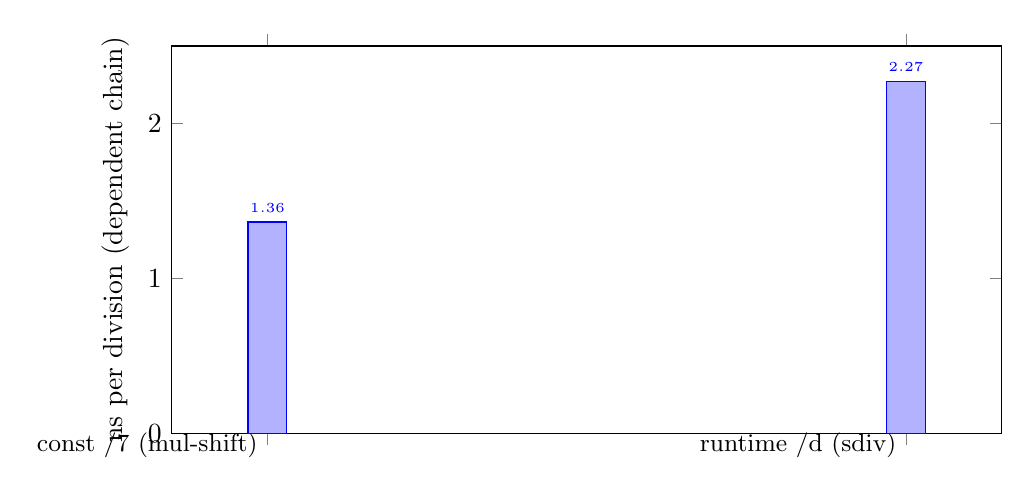
\begin{tikzpicture}
\begin{axis}[ybar, width=\textwidth, height=6.5cm, bar width=14pt, ymin=0, symbolic x coords={const /7 (mul-shift),runtime /d (sdiv)}, xtick=data, x tick label style={rotate=0, anchor=east, font=\small}, ylabel={ns per division (dependent chain)}, enlarge x limits=0.15, legend style={font=\small, at={(0.98,0.98)}, anchor=north east}, nodes near coords, nodes near coords style={font=\tiny}, every node near coord/.append style={/pgf/number format/.cd, fixed, precision=2}]
\addplot+[error bars/.cd, y dir=both, y explicit] coordinates {(const /7 (mul-shift),1.3635) +- (0,0.0020) (runtime /d (sdiv),2.2698) +- (0,0.0018)};
\end{axis}
\end{tikzpicture}